
\section{企业产能上限优化}

题目中要求在供应商和转运商有限的情况下,评估企业每周产能的上限。
本题在取消生产企业每周产能上限的同时,也消除了原材料的库存问题,这使得供应商和转运商的供应量可直接由生产企业转化为产能。
本问题也转化为在供应商和转运商有限的情况下,求供应链可向企业输送的最大供给量。

联系附件数据,我们得知近5 年来,共有402 家供应商通过8家转运商向企业供货。
而通过分析供货数据我们发现,每周转运商的总转运能力远少于供给商的供给能力,故向企业输送的最大供给量主要取决于转运商的转运能力。
因此,本模型主要对转运商的转运能力进行优化。

本文引申一家供应商每周供应的原材料尽量由一家转运商运输,提出运筹目标为参与转运的转运商次最少:
\begin{equation}
\begin{array}{l}
\min \sum_{j=1}^{402} \sum_{l=1}^{8}\left[\frac{\theta_{i j l}}{\psi_{i j}}\right] \\
\text { s.t. }\left\{\begin{array}{l}
\sum_{i=1}^{8} \theta_{i j l}=\psi_{i j} \\
\sum_{j=1}^{402} \theta_{i j l}=6000
\end{array}\right.
\end{array}
\end{equation}
式中,$[]$是高斯函数,代表向下取整;$\theta_{i j l}$是第$i$周转运商T$l$为供应商S$j$运输的供货量。
为保证企业产能充分发挥,约束了每家转运商均取得其最大转运能力6000立方米。

事实上,由于A类原材料生产商品的能力能力最强,企业此时仍对其表现出明显的偏好。

\begin{center} {\centering
\vbox{

    \centerline{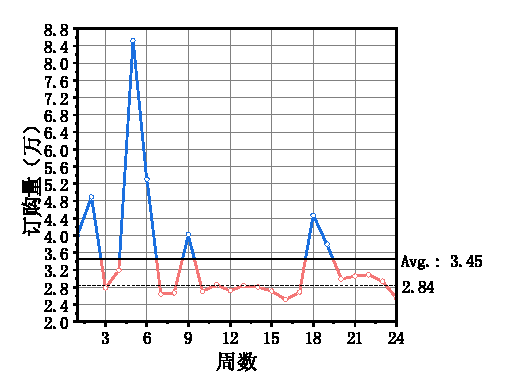
\includegraphics[width=8cm]{Image/qus_3_订购方案.eps}}
    \vskip 1mm{\small
    图9\quad 企业总订购量变化.
    \\}
    }
    }
\end{center}

由图可知,企业每周对A类原材料的收购量均为48000立方米,即为转运商的最大转运能力,符合转运商是生产限速步骤的预期。
而库存量严格维持为刚好满足企业两周生产需求的原材料库存量,说明提高产能还可以降低仓储成本,体现了科技作为第一生产力的重要地位。
但每周的转运商次变化较大,说明本模型能够有效安排转运商的运输工作,实施效果良好。

\section{模型的推广}

\subsection{模型的优点}
\begin{enumerate}
\item 建立了基于熵权逼近理想解方法的供应商排序模型,提高了综合评价的准确性和客观性。
\item 运用LSTM模型预测供货商的供应情况,从更深层次反映供货商实际供货情况。
\item 设计了使用计算机模拟供应过程的相关程序,运用仿真方法体现出优化方案的实际效果。
\end{enumerate}

本文中,对合作厂商先挑选再优化的办法可推广到其他商业合作中,进一步解决经济学和管理学中的许多问题,同时为社会学中的人际关系研究提供全新思路和不同视角;对企业生产成本进行优化来得到最经济方案的规划方法能给企业经营以理论指导,有很强的实践价值。
